\documentclass[11pt,aspectratio=1610,xcolor=dvipsnames]{beamer}

\usetheme[
    background=light,
    numbering=fraction,
    block=fill,
    progressbar=frametitle
]{metropolis}

\usepackage{physics}
\usepackage{bbm}
\usepackage[most]{tcolorbox}
\tcbset{variables/.style={colback=yellow!20,colframe=yellow}}
\usepackage{tikz}
\usetikzlibrary{arrows}
\usetikzlibrary{shapes.geometric, arrows, shadows}
\usetikzlibrary{fit, backgrounds}
% \colorlet{LightLavender}{Lavender!40!}
\newtcolorbox{prob}{colback=red!5!white,colframe=red!75!black}
\usefonttheme[onlymath]{serif}
\usepackage{quantikz}
\usepackage{qrcode}
\usepackage{pgfplots}

% todonotes hack
\usepackage{xkeyval}
\usepackage{todonotes}
\presetkeys{todonotes}{inline}{}

\newcommand{\R}{\mathbb{R}}
\newcommand{\U}[1]{\mathsf{U}(#1)}
\newcommand{\defeq}{\stackrel{\text{\tiny def}}{=}}
\def\Put(#1,#2)#3{\leavevmode\makebox(0,0){\put(#1,#2){#3}}}


\title{Error Mitigation with Mitiq}
\date{Sep 18, 2023}
\author{Nate Stemen}
\institute{
\includegraphics[width=0.3\textwidth]{unitary_fund_logo.png}\\[\medskipamount]

\includegraphics[width=0.3\textwidth]{team.png}}


\begin{document}

\maketitle

\begin{frame}{Mitiq}
	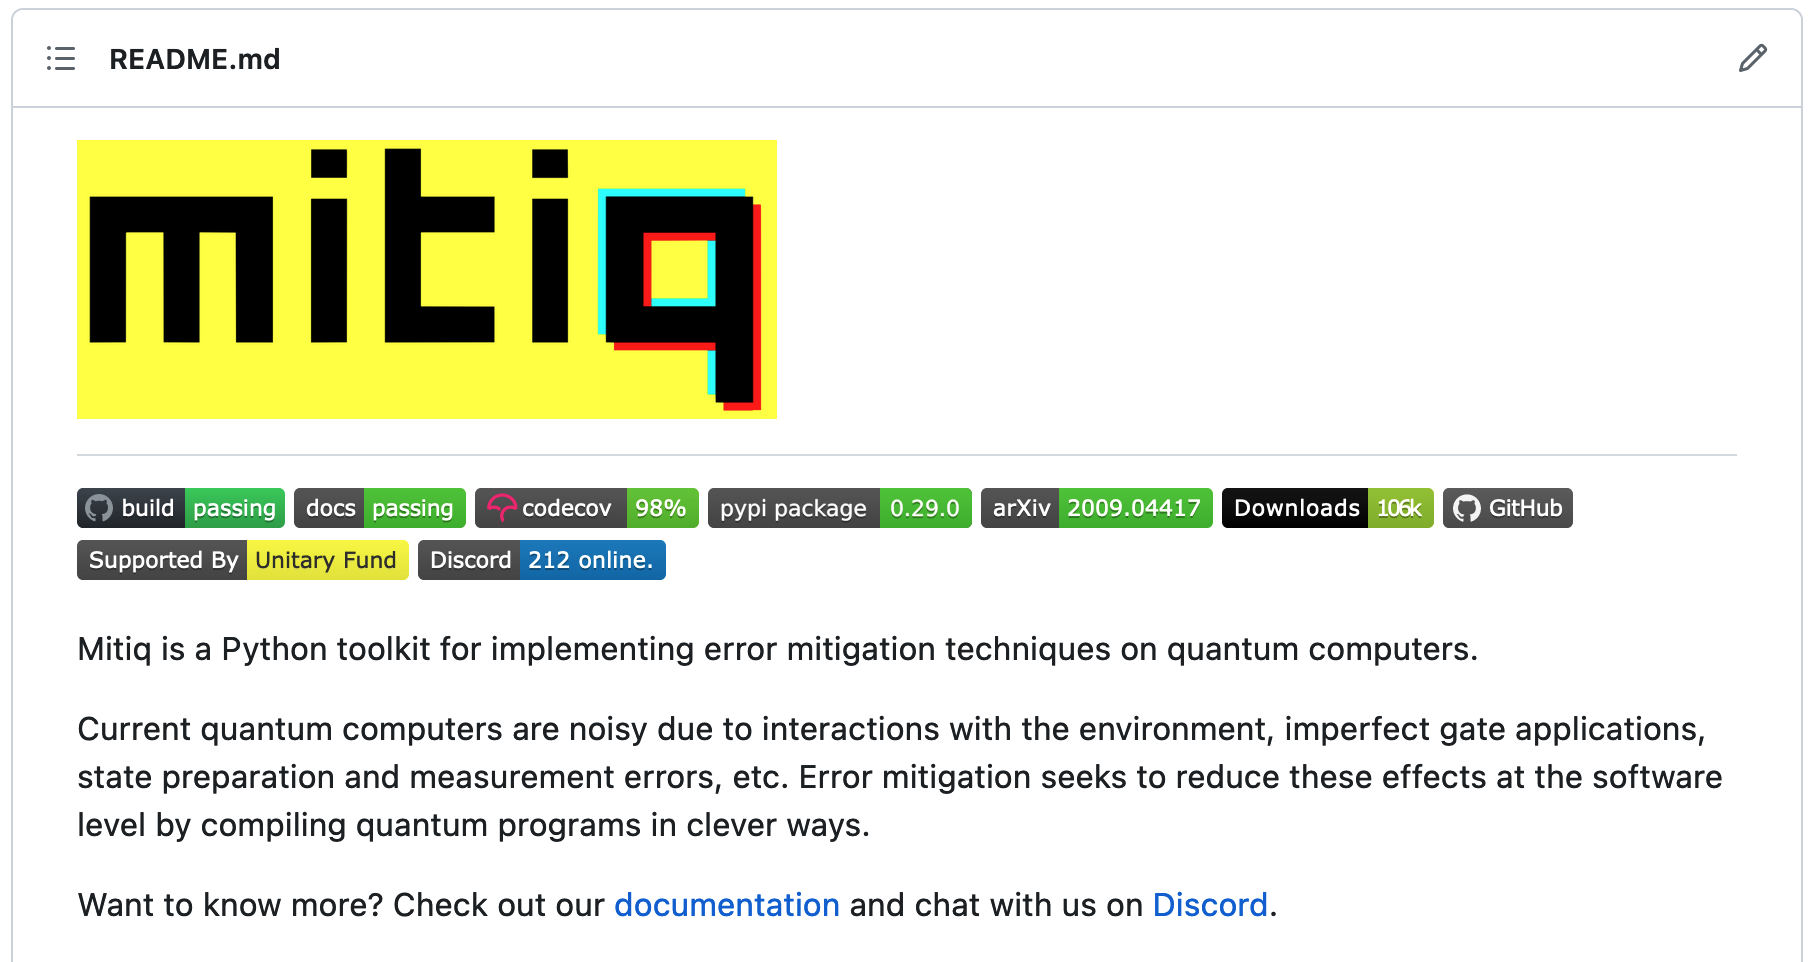
\includegraphics[width=0.6\textwidth]{mitiq.png}
	\pause
	\Put(-150, 10){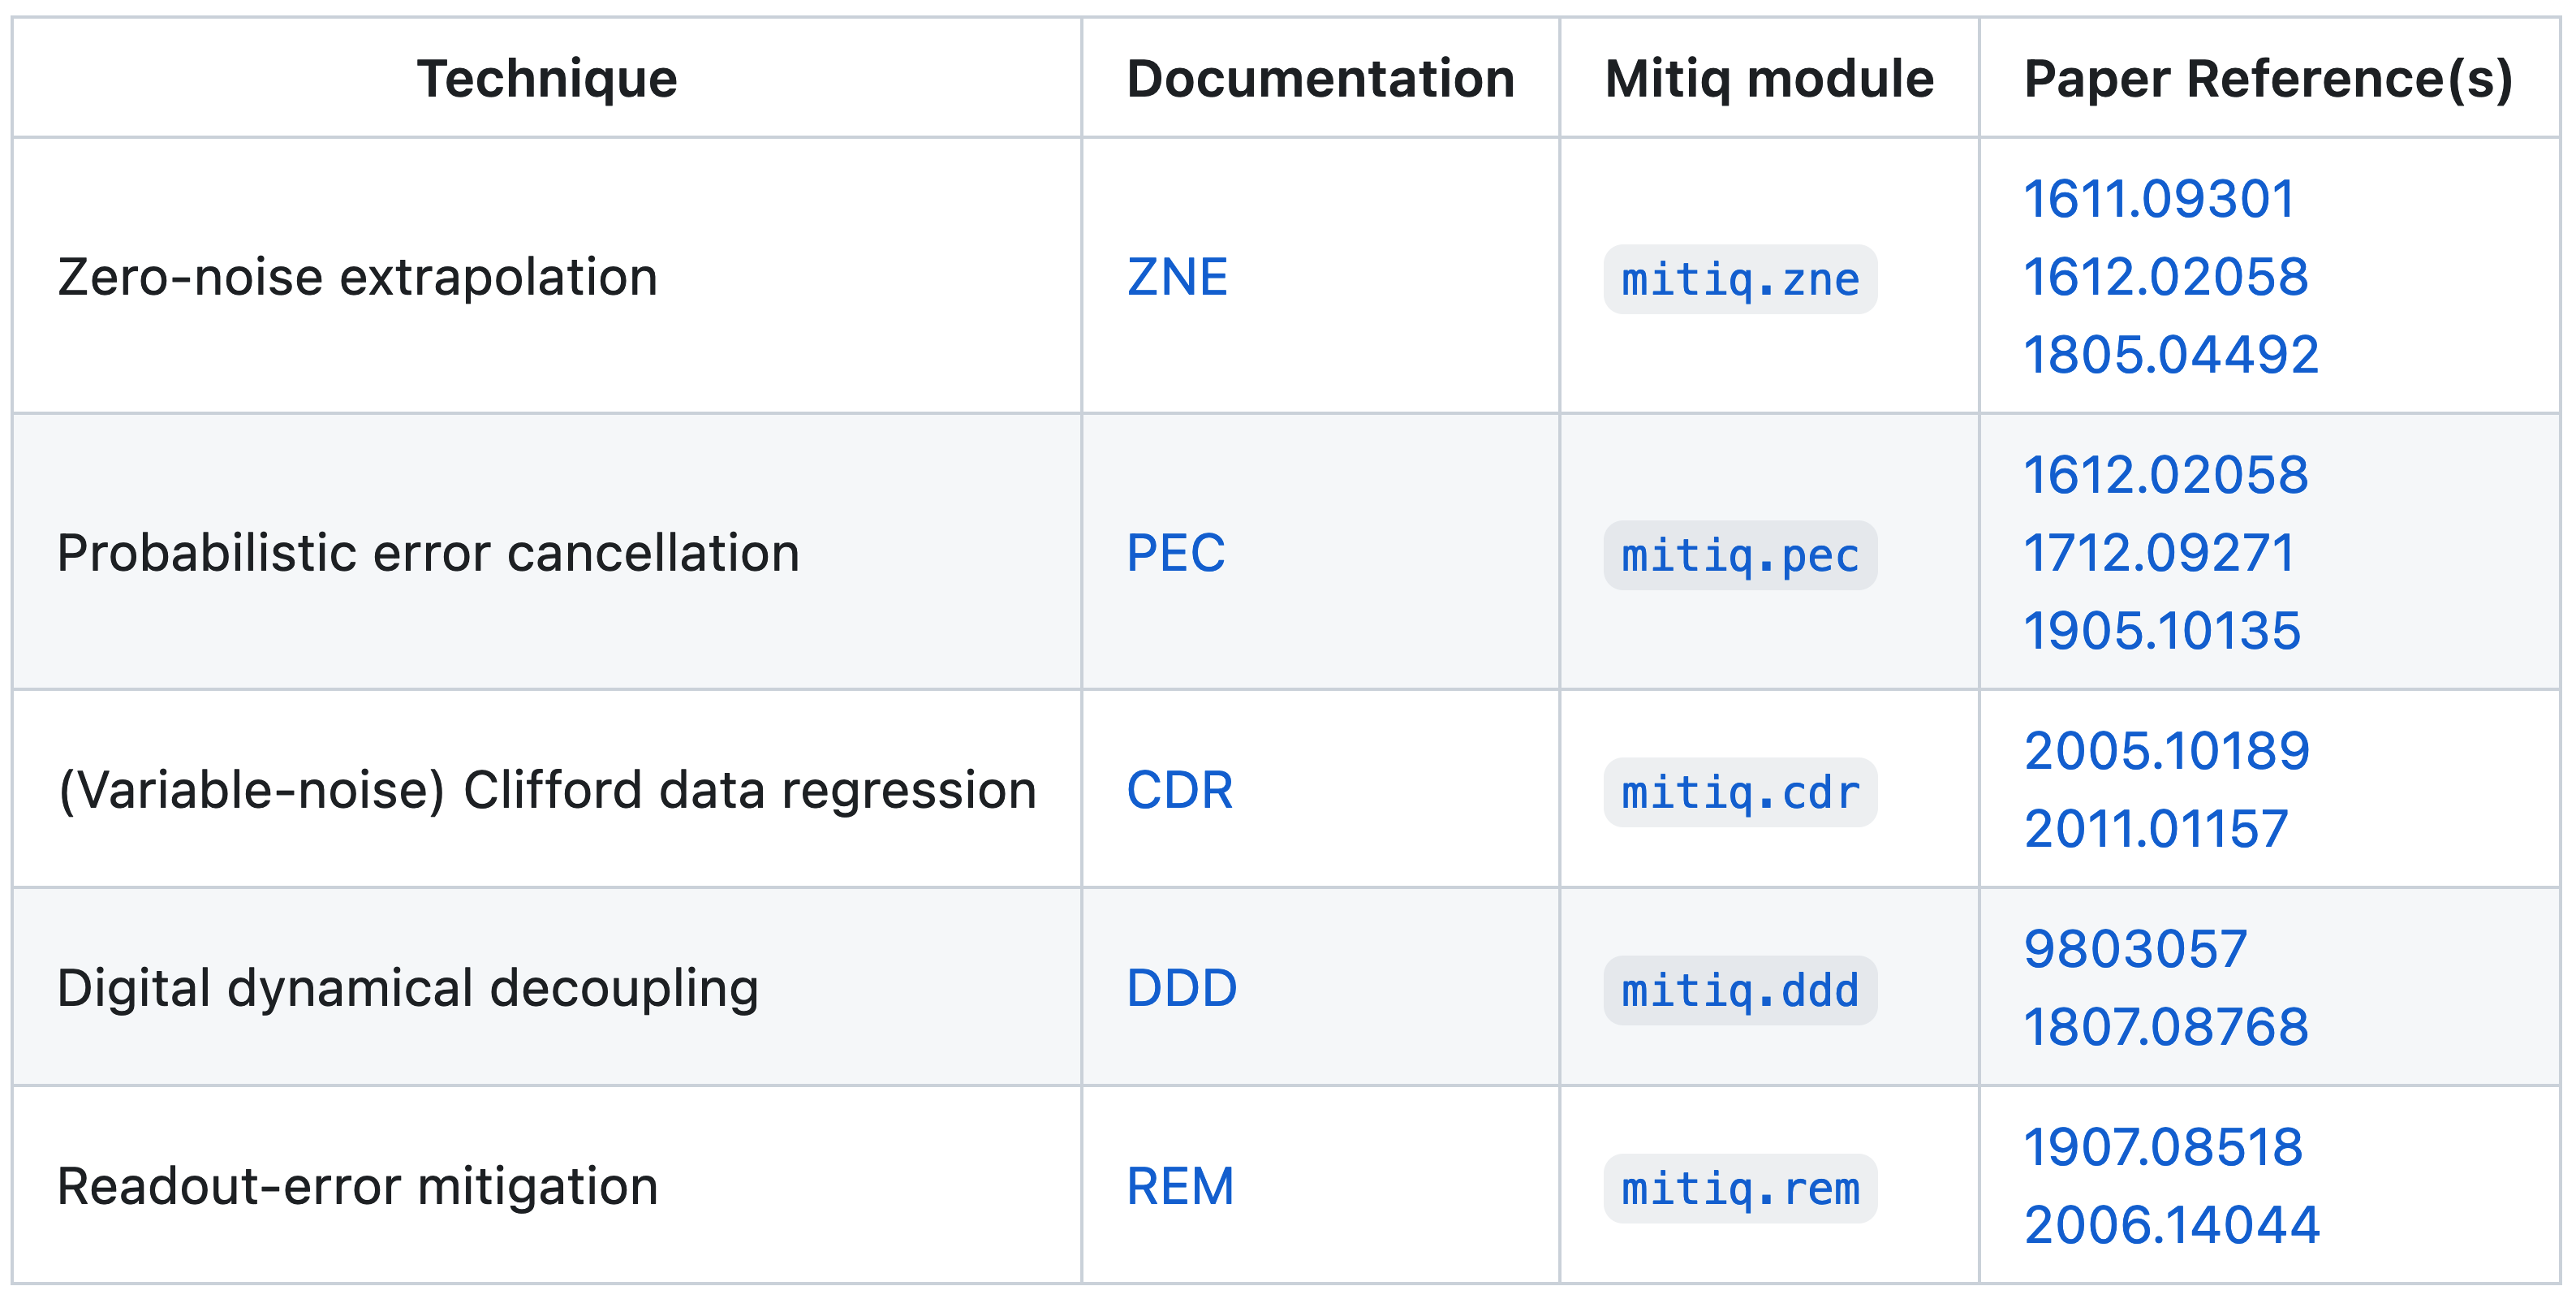
\includegraphics[width=0.6\textwidth]{techniques.png}}
	\pause
	\Put(-70, 170){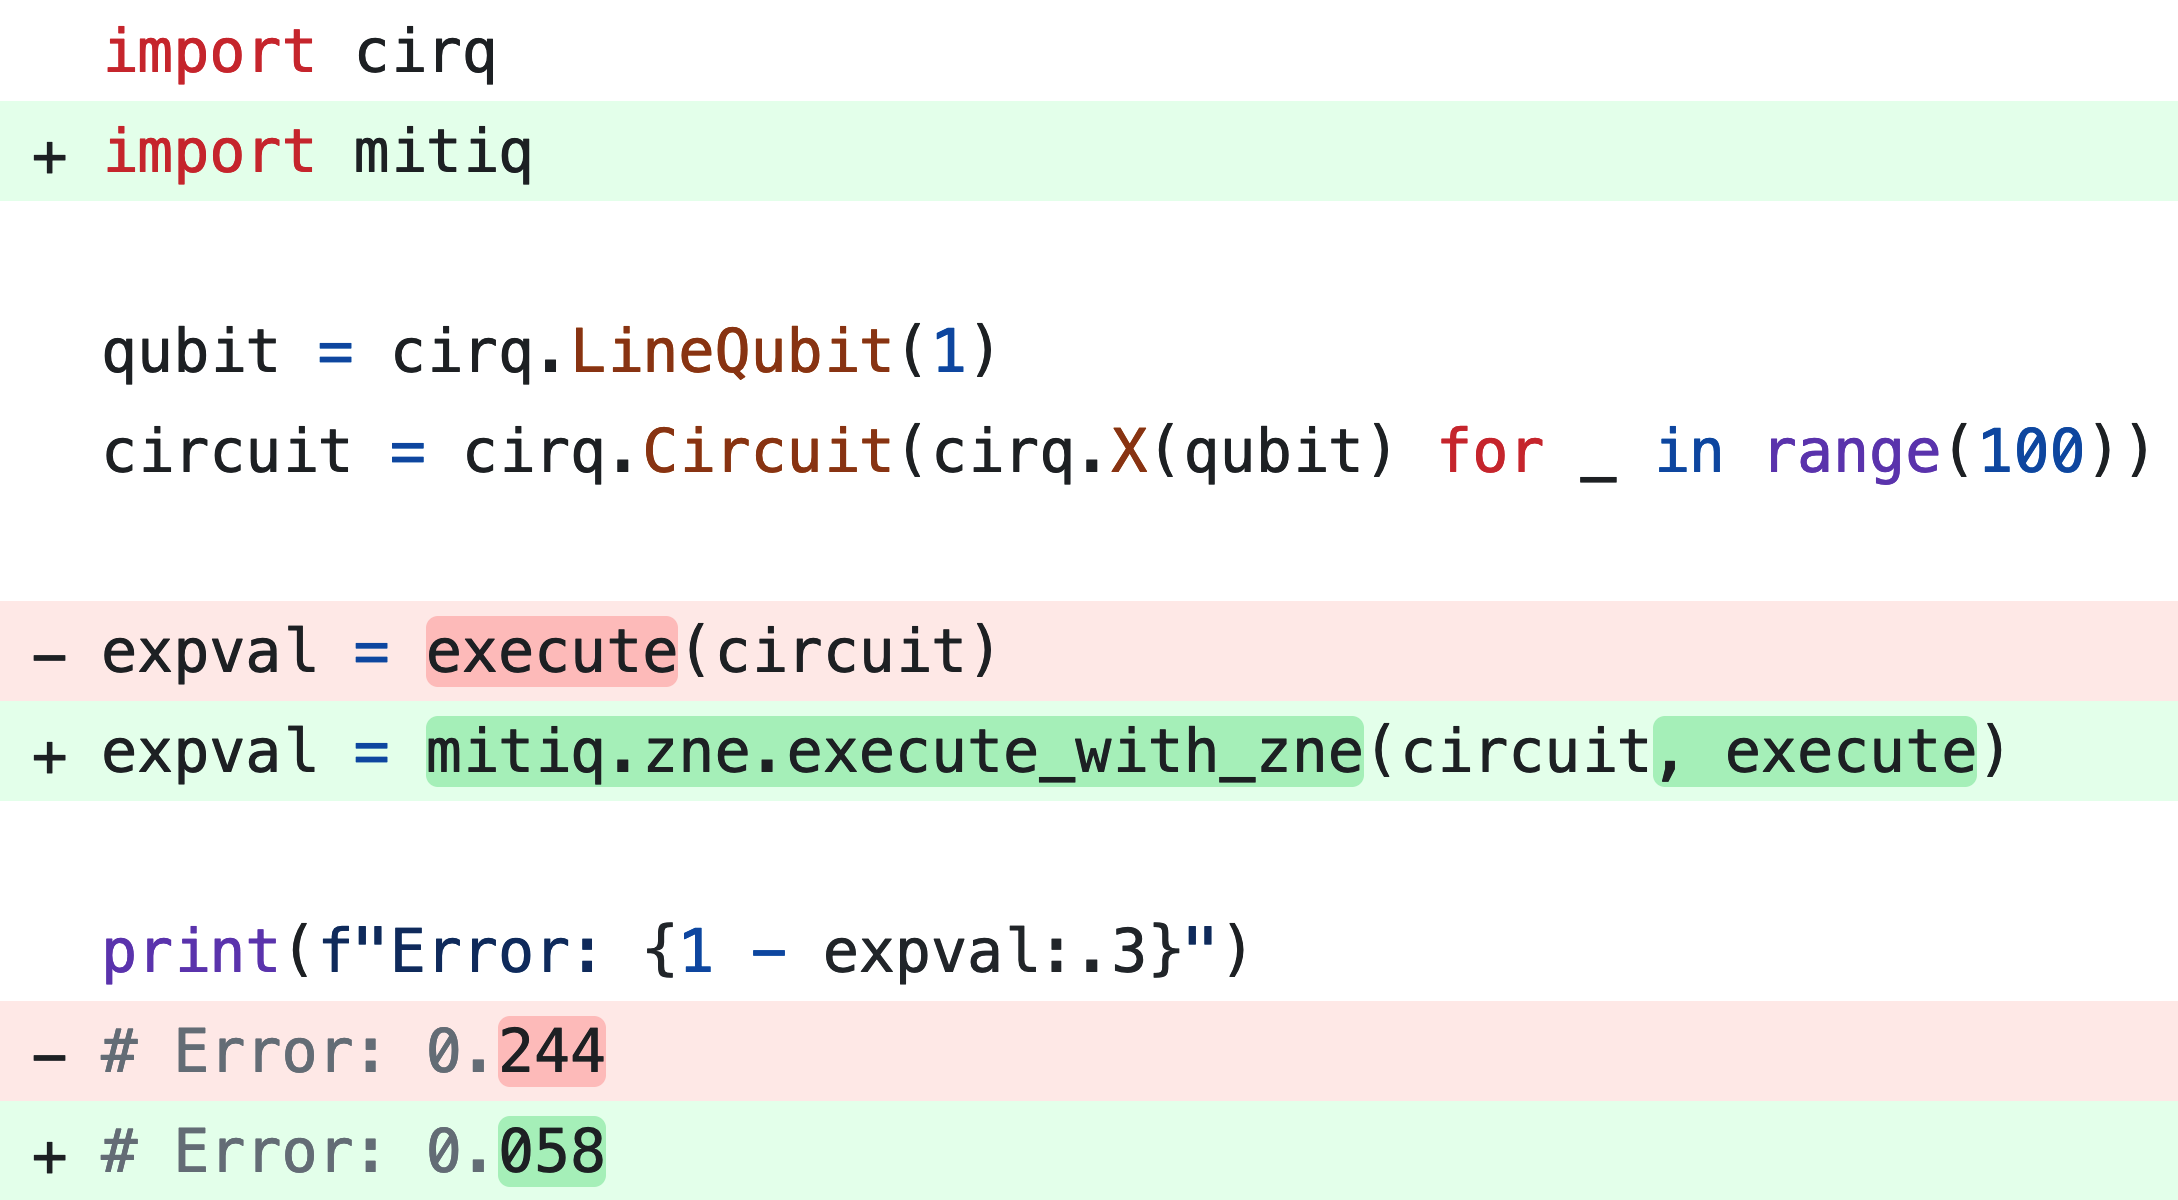
\includegraphics[width=0.6\textwidth]{inaction.png}}
	\pause
	\Put(120, 260){
\includegraphics[width=0.12\textwidth]{cirq.png}}
	\pause
	\Put(120, 160){
\includegraphics[width=0.11\textwidth]{qiskit.png}}
	\Put(115, 70){
\includegraphics[width=0.11\textwidth]{pennylane.png}}
	\Put(120, -50){
\includegraphics[width=0.09\textwidth]{pyquil.png}}
	\Put(110, -130){
\includegraphics[width=0.11\textwidth]{braket.png}}
\end{frame}

\begin{frame}{Follow along!}
	\begin{center}
		\qrcode[height=5cm]{https://github.com/unitaryfund/mitiq-tutorial/}

		\url{https://github.com/unitaryfund/mitiq-tutorial}
	\end{center}
\end{frame}

\begin{frame}{Experience}
	\begin{enumerate}[<+->]
		\item Who has written a quantum program before?
		\item Who has run a quantum program on hardware before?
		\item Who has used error mitigation?
		\item Who has used Mitiq?
	\end{enumerate}
\end{frame}

\begin{frame}{Tutorial goals}
	\begin{enumerate}
		\item Understand context, and general ideas of quantum error mitigation (QEM).
		\item Understand main ideas of ZNE, PEC, and DDD along with pros and cons of each technique.
		\item Ability to use Mitiq to apply these techniques in a quantum pipeline.
	\end{enumerate}
\end{frame}

\begin{frame}{What is Quantum Error Mitigation?}
	\begin{block}{Quantum Error Mitigation}
		The acceptance that available quantum devices are noisy\ldots maybe very much so.
		But we still want to use them!
	\end{block}
	\begin{columns}
		\uncover<2->{
			\begin{column}{0.35\textwidth}
				\begin{itemize}[<+->]
					\item (In)coherent noise
					\item SPAM errors
					\item Crosstalk
					\item Calibration errors
					\item \dots
				\end{itemize}
			\end{column}
		}
		\uncover<+->{
			\begin{column}{0.6\textwidth}
				\begin{center}
					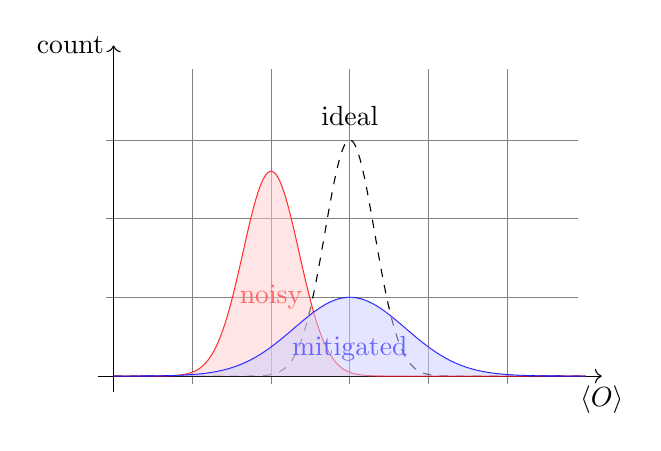
\begin{tikzpicture}[domain=0:6, samples=200]
						\draw[very thin,color=gray] (-0.1,-0.1) grid (5.9,3.9);

						\draw[->] (-0.2,0) -- (6.2,0) node[below] {$\langle O\rangle$};
						\draw[->] (0,-0.2) -- (0,4.2) node[left] {count};

						\draw[dashed, color=black] plot (\x,{3*exp(-5*(\x - 3)^2)}) node[right] {};
						\node at (3, 3.3) {ideal};

						\uncover<+->{
							\draw[color=red] plot (\x,{2.6*exp(-4*(\x - 2)^2)}) node[above] {};
							\node[color=red] at (2,1) {noisy};
							\fill[fill=red!20, opacity=0.5] plot (\x,{2.6*exp(-4*(\x - 2)^2)});
						}

						\uncover<+->{
							\draw[color=blue] plot (\x,{exp(-1*(\x - 3)^2)}) node[right] {};
							\node[color=blue] at (3,0.35) {mitigated};
							\fill[fill=blue!20, opacity=0.5] plot (\x,{exp(-1*(\x - 3)^2)});
						}
					\end{tikzpicture}
				\end{center}
			\end{column}
		}
	\end{columns}
\end{frame}

\begin{frame}{QEM Methods}
	\begin{columns}[T]
		\begin{column}{0.33\textwidth}
			\begin{tcolorbox}[title=Zero-Noise\\Extrapolation,halign title=center,halign=center,colback=PineGreen!20, colframe=PineGreen!70]
				\vspace{-.5cm}
				\begin{equation*}
					\partial_t \rho = -i \comm{H}{\rho} + \tcbhighmath[left=0mm, right=0mm, top=0mm, bottom=0mm, colback=yellow!30!white, boxrule=0mm]{\lambda} \mathcal{L}(\rho)
				\end{equation*}
			\end{tcolorbox}
			\begin{tcolorbox}[title=Symmetry-based techniques,halign title=center,halign=center,colback=gray!20, colframe=gray!70]
				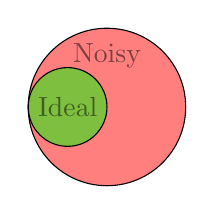
\begin{tikzpicture}
					\begin{scope}[fill opacity=0.5]
						\draw[fill=red, draw = black] (0,0) circle (1);
						\draw[fill=green, draw = black] (-.5,0) circle (.5);
						\node at (0,0.65) (A) {Noisy};
						\node at (-.5,0) (B) {Ideal};
					\end{scope}
				\end{tikzpicture}
				\vspace{-.5cm}
				\begin{align*}
					M \ket{\psi} & = \ket{\psi}                  \\
					\rho         & = \frac{M \rho M}{\tr(M\rho)}
				\end{align*}
			\end{tcolorbox}
		\end{column}
		\begin{column}{0.33\textwidth}
			\begin{tcolorbox}[title=Probabilistic Error Cancellation,halign title=center,halign=center,colback=PineGreen!20, colframe=PineGreen!70]
				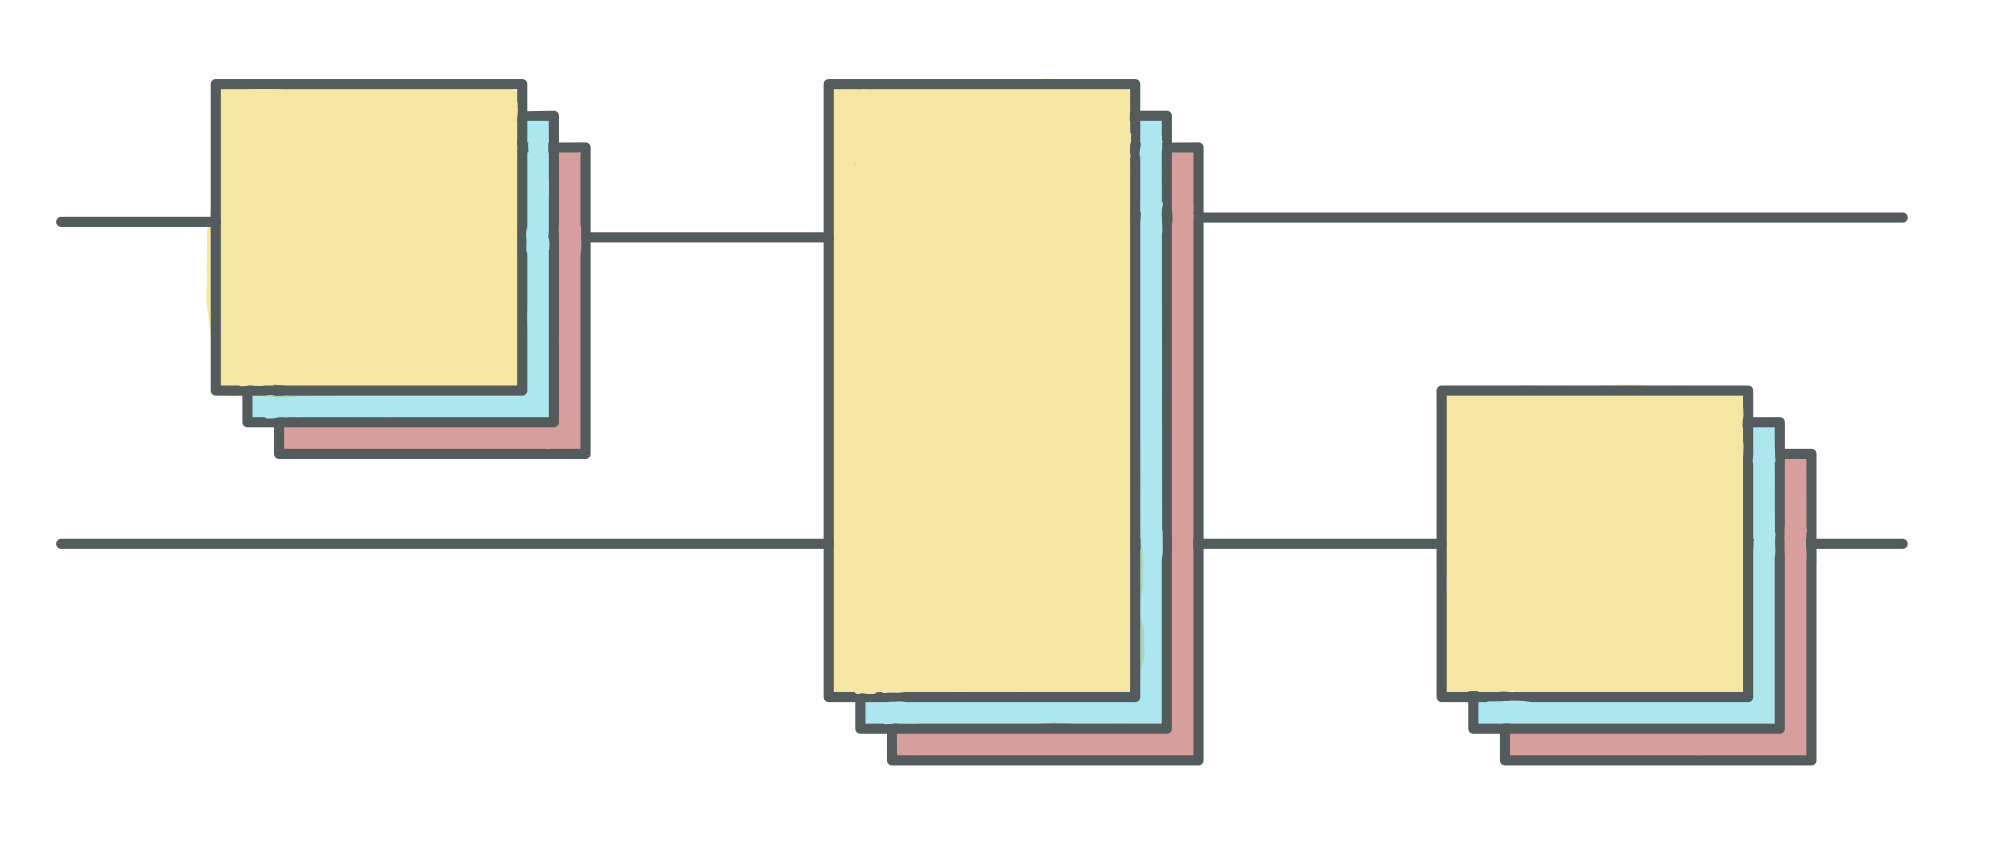
\includegraphics[width=\textwidth]{peccircuits.jpeg}
			\end{tcolorbox}
			\begin{tcolorbox}[title=Dynamical Decoupling,halign title=center,halign=center,colback=PineGreen!20, colframe=PineGreen!70]
				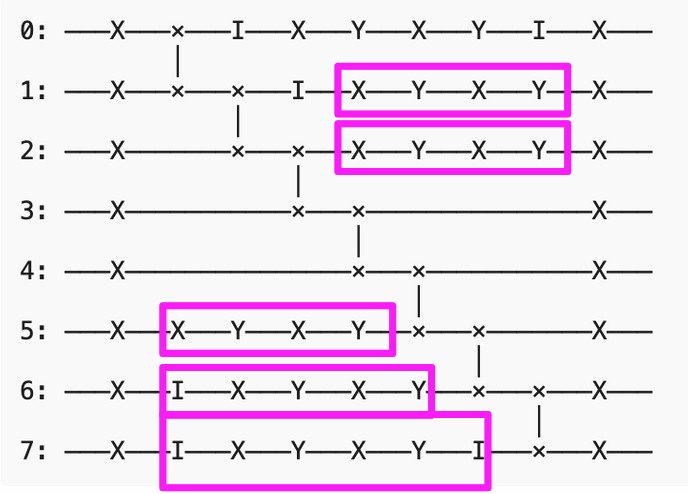
\includegraphics[width=\textwidth]{dd.png}
			\end{tcolorbox}
		\end{column}
		\begin{column}{0.33\textwidth}
			\begin{tcolorbox}[title=Learning-based methods,halign title=center,halign=center,colback=gray!20, colframe=gray!70]
				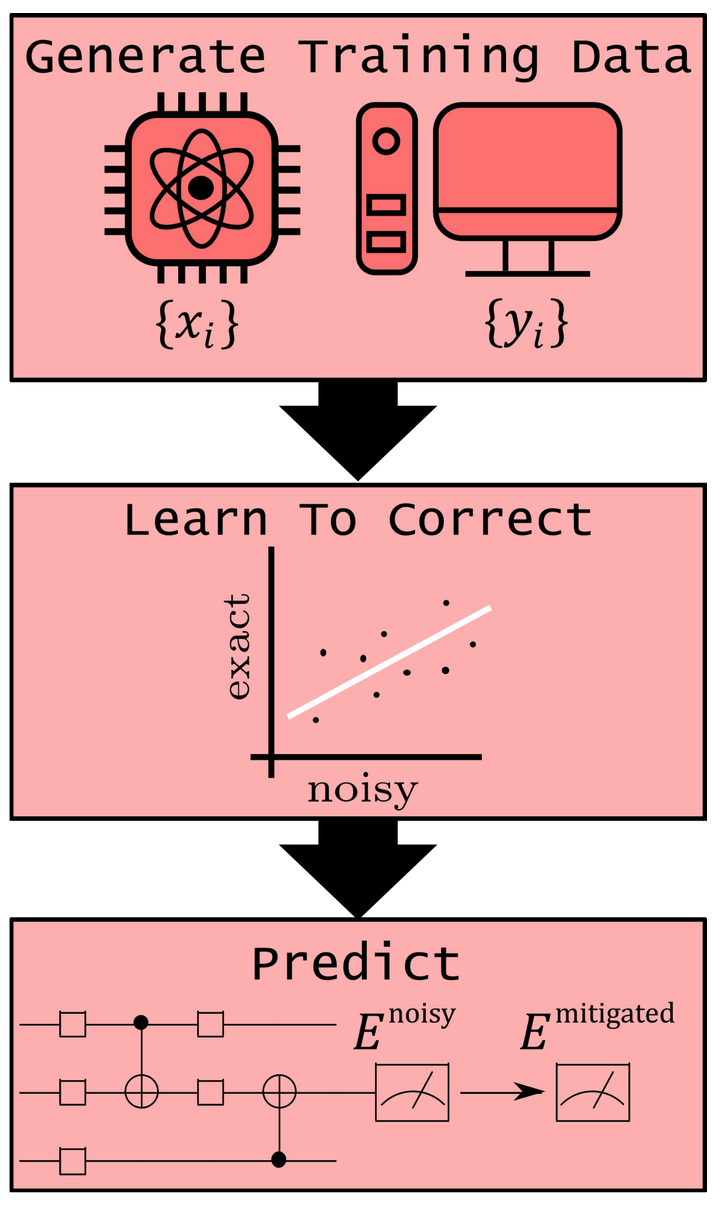
\includegraphics[width=\textwidth]{learning-based.png}
			\end{tcolorbox}

		\end{column}
	\end{columns}
\end{frame}

\begin{frame}{What about error correction?}
	\begin{figure}[h]
		\centering
		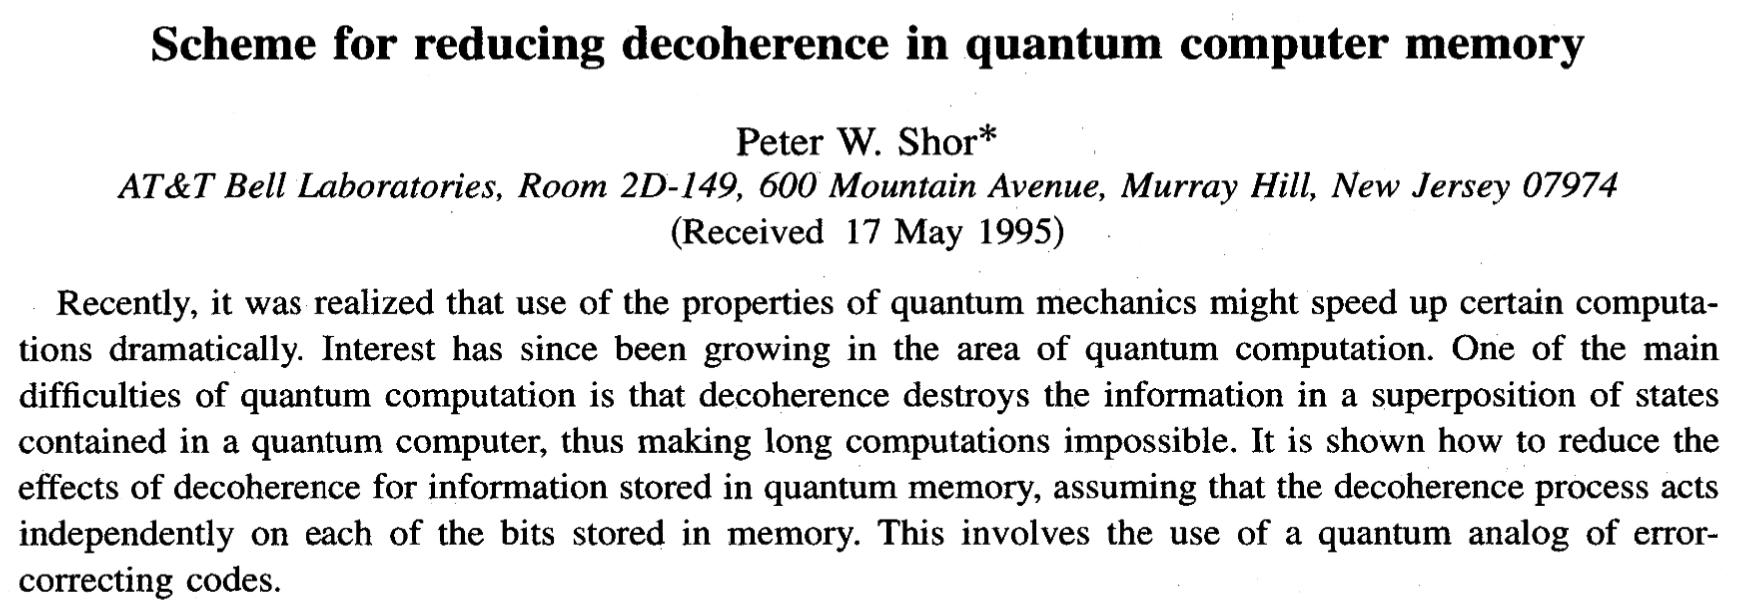
\includegraphics[width=.7\textwidth]{shor-qec.png}
		\note{first by shor, but also Steane and Calderbank in the years after refining the 9-qubit Shor code}
	\end{figure}
	\begin{columns}[t]
		\begin{column}{0.5\textwidth}
			\uncover<2->{
				\begin{block}{Error Correction}
					\begin{itemize}
						\item Encode logical qubits into many physical qubits
						\item Intermediate measurements produce syndromes
						\item Use syndromes to correct errors
					\end{itemize}
				\end{block}
			}
			\uncover<4->{
				\begin{tikzpicture}[overlay]
					\node[draw=none, fill=yellow, rotate=20, minimum width=5cm, minimum height=1cm] at (3.5, 2.5) {Scalable, but unfeasible};
				\end{tikzpicture}
			}
		\end{column}
		\begin{column}{0.5\textwidth}
			\uncover<3->{
				\begin{block}{Error Mitigation}
					\begin{itemize}
						\item Perform multiple and different noisy computations
						\item Collect results
						\item Infer ideal expectation values
					\end{itemize}
				\end{block}
			}
			\uncover<5->{
				\begin{tikzpicture}[overlay]
					\node[draw=none, fill=yellow, rotate=20, minimum width=5cm, minimum height=1cm] at (3.5, 1.95) {Unscalable$^*$, but feasible};
				\end{tikzpicture}
			}
		\end{column}
	\end{columns}
\end{frame}

\begin{frame}{Zero-Noise Extrapolation (ZNE)}

	\begin{exampleblock}{Key Idea}<+->
		Scale noise up, extrapolate back to zero-noise value.
	\end{exampleblock}

	\begin{columns}
		\begin{column}{0.4\textwidth}
			\uncover<+->{
				\vspace{-2cm}
				\begin{equation*}
					\partial_t \rho = - i \comm{H}{\rho} + \lambda \mathcal{L}(\rho)
				\end{equation*}
			}
			\vspace{-1cm}
			\begin{center}
				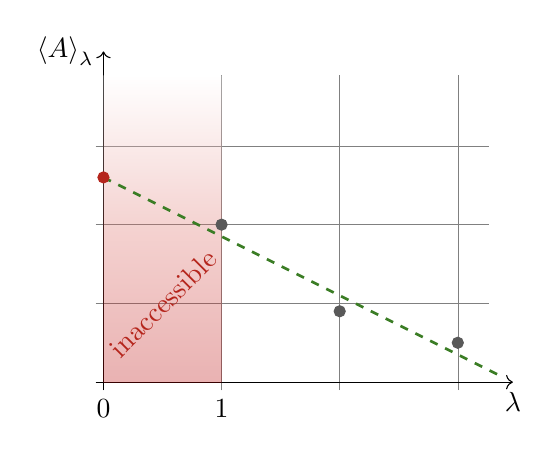
\begin{tikzpicture}
					\uncover<+->{
						\draw[very thin,color=gray] (-0.1,-0.1) grid [xstep=1.5] (4.9, 3.9);

						\draw[->] (-0.1,0) -- (5.2,0) node[below] {$\lambda$};
						\draw[->] (0,-0.1) -- (0,4.2) node[left] {$\expval{A}_\lambda$};
						\fill (0, -0.1)   circle[radius=0pt] node[below] {$0$};
						\fill (1.5, -0.1) circle[radius=0pt] node[below] {$1$};
					}

					\uncover<+->{
						\draw[bottom color=BrickRed, top color=white,opacity=0.3, draw=none] (0,0) rectangle (1.5, 3.9);
					}
					\only<4>{\node[rotate=45, color=BrickRed] at (0.75, 1) {inaccessible};}

					\uncover<+->{
						\filldraw[gray!70!black] (1.5,2) circle (2pt);
					}
					\uncover<+->{
						\filldraw[gray!70!black] (3,  0.9) circle (2pt);
						\filldraw[gray!70!black] (4.5,0.5) circle (2pt);
					}
					\uncover<+->{
						\draw[dashed, domain=0:5, variable=\x, OliveGreen, line width=1pt] plot ({\x}, {-0.5*\x + 2.6});
					}
					\uncover<+->{
						\filldraw[BrickRed] (0,2.6) circle (2pt);
					}
				\end{tikzpicture}
			\end{center}
		\end{column}

		\begin{column}{0.6\textwidth}
			\uncover<+->{How do we scale the noise \textbf{up}?}
			\uncover<+->{
				\begin{center}
					\begin{tikzpicture}
						\begin{axis}[ymin=0, ymax=10, xmin=-.5, xmax=16.5, tiny, axis y line=left, ytick=\empty, axis x line=bottom, xtick=\empty, xlabel=$t$, ylabel=Pulse strength]
							\addplot[blue, ultra thick] table {pulse.dat};
						\end{axis}
					\end{tikzpicture}%
					\quad
					\begin{tikzpicture}
						\begin{axis}[x=.25cm, ymin=0, ymax=10, xmin=-.5, xmax=16.5, tiny, axis y line=left, ytick=\empty, axis x line=bottom, xtick=\empty, xlabel=$t$]
							\addplot[blue, ultra thick] table {pulse-squish.dat};
						\end{axis}
					\end{tikzpicture}%
				\end{center}
			}
			\begin{columns}[onlytextwidth]
				\begin{column}{0.5\textwidth}
					\vspace{3cm}
					\uncover<10->{
						\begin{quantikz}
							& \gate{} & \gate[2]{}  & \qw     & \qw \\
							& \qw     &             & \gate{} & \qw
						\end{quantikz}
					}
				\end{column}
				\begin{column}[t]{0.5\textwidth}
					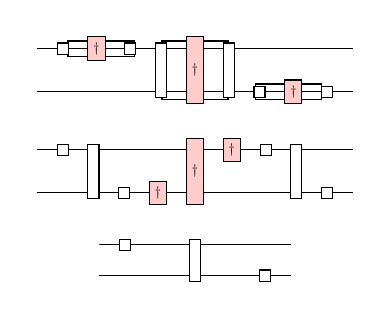
\begin{tikzpicture}
						\only<10>{
							\node[scale=.7] {
								\begin{quantikz}
									& \gate[][1.2cm]{} & \gate[2][1.2cm]{} & \qw              & \qw \\
									& \qw              &                   & \gate[][1.2cm]{} & \qw
								\end{quantikz}
							};
						}
						\uncover<+->{
							\node[scale=.5] (local) {
								\begin{quantikz}
									& \gate{} & \gate[style={fill=red!20}]{\dagger} & \gate{} & \gate[2]{} & \gate[2, style={fill=red!20}]{\dagger} & \gate[2]{} & \qw     & \qw                          & \qw     & \qw \\
									& \qw     & \qw                          & \qw     &            &                                 &            & \gate{} & \gate[style={fill=red!20}]{\dagger} & \gate{} & \qw
								\end{quantikz}
							};
							\node[scale=.5, below=.2cm of local] (global) {
								\begin{quantikz}
									& \gate{} & \gate[2]{}  & \qw     & \qw     & \gate[2, style={fill=red!20}]{\dagger} & \gate[style={fill=red!20}]{\dagger} & \gate{} & \gate[2]{}  & \qw     & \qw \\
									& \qw     &             & \gate{} & \gate[style={fill=red!20}]{\dagger} &            & \qw     & \qw     &             & \gate{} & \qw
								\end{quantikz}
							};
							\node[scale=.5, below=.2cm of global] (ii) {
								\begin{quantikz}
									& \gate{} & \qw & \qw & \gate[2]{} & \qw & \qw & \qw     & \qw \\
									& \qw     & \qw & \qw &            & \qw & \qw & \gate{} & \qw
								\end{quantikz}
							};
						}
					\end{tikzpicture}
				\end{column}
			\end{columns}
		\end{column}
	\end{columns}
\end{frame}

\tikzset{rect/.style={rectangle, rounded corners, minimum width=3.5cm,
			minimum height=1cm, text centered, draw=Cerulean!50, fill=Cerulean!10},
	arrow/.style={thick,->,>=stealth}}

\begin{frame}{Running quantum programs in practice}
	\begin{center}
		\begin{tikzpicture}%[node distance=2cm]

			\node (qp) [rect] {Quantum Program};
			\node (backend) [rect, right = 1cm of qp] {Execute};
			\node (result) [rect, below = 1.50cm  of qp] {Results};

			\draw [arrow] (qp) -- (backend);
			\draw [arrow] (backend) |- (result);
			\coordinate (aux) at (result.south -| backend);
			\coordinate (aux2) at (qp.north -| backend);

			\begin{scope}[on background layer]
				\node[draw, dashed, gray, rounded corners, fill=red!20, fit=(qp) (result), label={above:User}]{};
				\node[draw, dashed, gray, rounded corners, fill=gray!50, fit=(backend) (aux) (aux2), label={above:Hardware/Simulator}]{};
			\end{scope}
		\end{tikzpicture}
	\end{center}
\end{frame}

\begin{frame}{Running quantum programs in practice with Mitiq}
	\begin{center}
		\begin{tikzpicture}%[node distance=2cm]

			\node (qp) [rect] {Quantum Program};

			\node (many) [rect, below right = -0.8cm and .7cm of qp] {};
			\node [rect, below right = -0.9cm and .6cm of qp] {};
			\node (circuits) [rect, right = .5cm of qp] {Intermediary circuits};

			\node (backend) [rect, right = .7cm of circuits] {Execute};

			\node [rect, below left = 1.3cm and .5cm of backend] {};
			\node [rect, below left = 1.4cm and .6cm of backend] {};
			\node (noisy) [rect, below left = 1.5cm and .7cm of backend] {Noisy results};

			\node (result) [rect, below = 1.50cm  of qp] {Results};

			\draw [arrow] (qp) -- (circuits);
			\draw [arrow] (circuits) -- (backend);
			\draw [arrow] (backend) |- (noisy);
			\draw [arrow] (noisy) -- (result);
			\coordinate (aux) at (result.south -| backend);
			\coordinate (aux2) at (qp.north -| backend);

			\begin{scope}[on background layer]
				\node[draw, dashed, gray, rounded corners, fill=red!20, fit=(qp) (result), label={above:User}]{};
				\node[draw, dashed, gray, rounded corners, fill=gray!50, fit=(backend) (aux) (aux2), label={above:Hardware/Simulator}]{};
				\node[draw, dashed, gray, rounded corners, fill=yellow!50, fit=(circuits) (many) (noisy), label={above:Error Mitigation}]{};
			\end{scope}
		\end{tikzpicture}
	\end{center}
\end{frame}

\begin{frame}{Let's try Mitiq!}
	\begin{center}
		\qrcode[height=5cm]{https://github.com/unitaryfund/mitiq-tutorial/}

		\url{https://github.com/unitaryfund/mitiq-tutorial/}
	\end{center}
\end{frame}

\begin{frame}[fragile]{Executors Continued}
	An executor is anything with a type signature:
	\begin{center}
		\texttt{(QPROGRAM -> QuantumResult)}
	\end{center}
	\vspace{1cm}
	\texttt{QPROGRAM} $ =
		\begin{array}{l}
			
\includegraphics[width=0.1\textwidth]{cirq.png}
		\end{array}
		\bigcup
		\begin{array}{l}
			
\includegraphics[width=0.1\textwidth]{qiskit.png}
		\end{array}
		\bigcup
		\begin{array}{l}
			
\includegraphics[width=0.09\textwidth]{pyquil.png}
		\end{array}
		\bigcup
		\begin{array}{l}
			
\includegraphics[width=0.11\textwidth]{braket.png}
		\end{array}
		\bigcup
		\begin{array}{l}
			
\includegraphics[width=0.12\textwidth]{pennylane.png}
		\end{array}
	$

	\texttt{QuantumResult} $ = \mathtt{float} \cup \mathtt{density} \cup \mathtt{bitstring}$
\end{frame}

\begin{frame}{Calibration}
\end{frame}

\begin{frame}[t]{Sneak Preview of Part II}
	\only<1>{
		\begin{exampleblock}{Probabilistic Error Cancellation}
			\textbf{Key Idea}: Use noisy operations to build up noiseless ones by selective cancellation and sampling.
		\end{exampleblock}
		\begin{figure}[h]
			\centering
			\includegraphics[width=0.7\textwidth]{pec_workflow.png}
		\end{figure}
	}

	\only<2>{
		\begin{exampleblock}{Digital Dynamical Decoupling}
			\textbf{Key Idea}: The devil finds work for idle [qubits].
		\end{exampleblock}
		\begin{figure}[h]
			\centering
			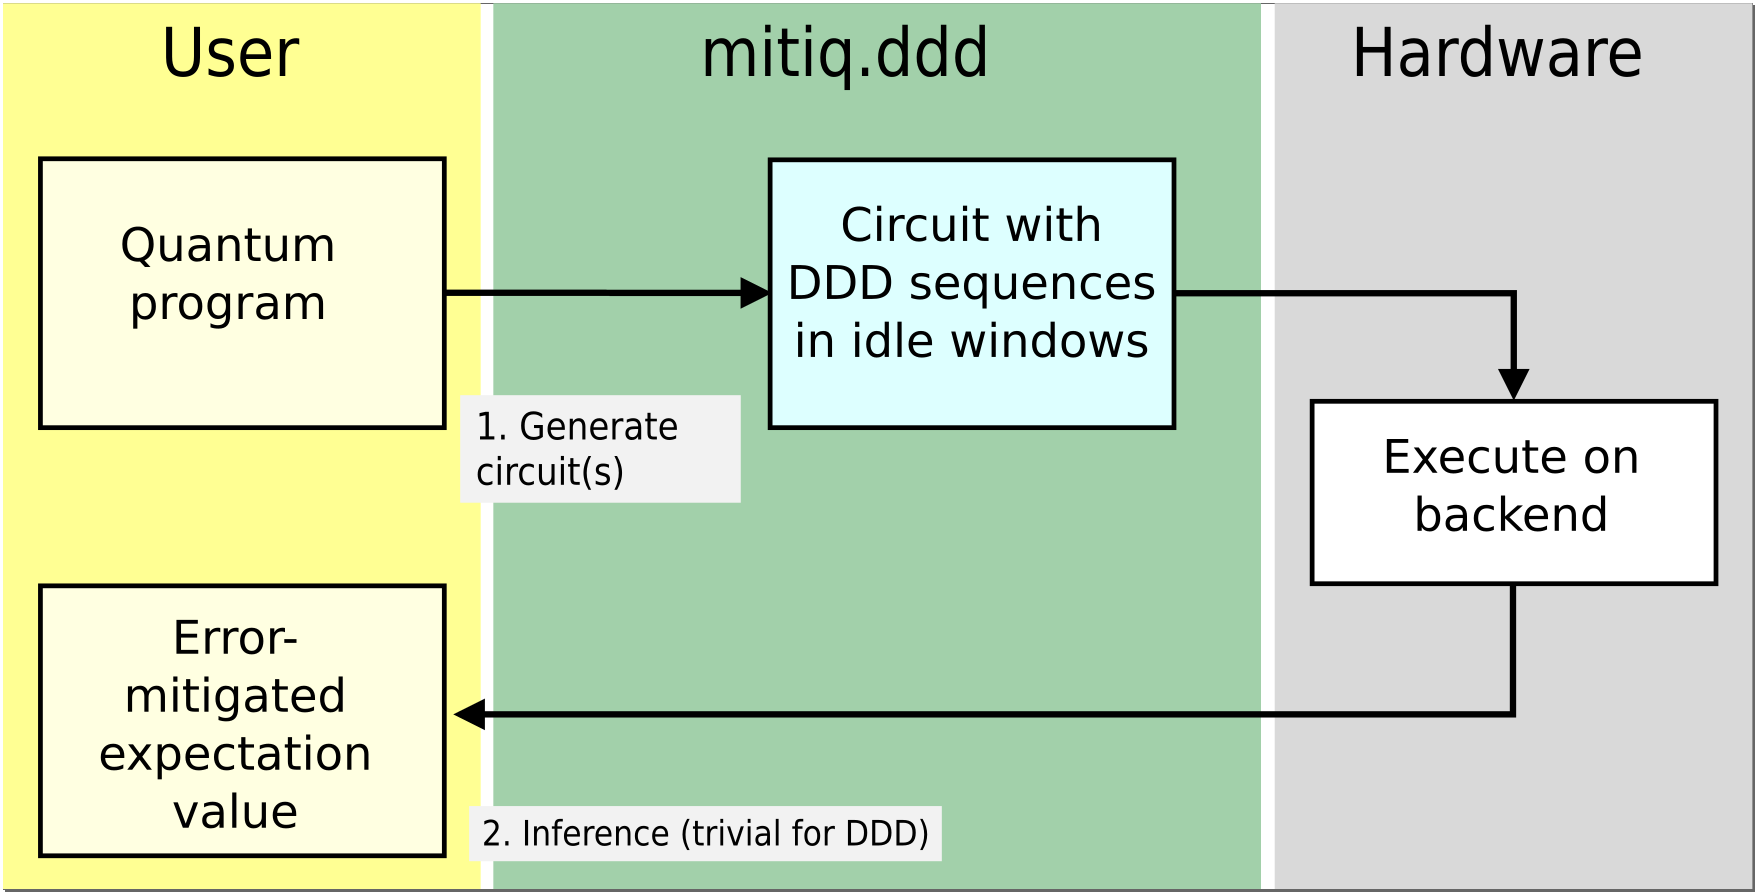
\includegraphics[width=0.7\textwidth]{ddd_workflow.png}
		\end{figure}
	}
\end{frame}

\begin{frame}{Interested in this work?}
	\begin{figure}[h]
		\centering
		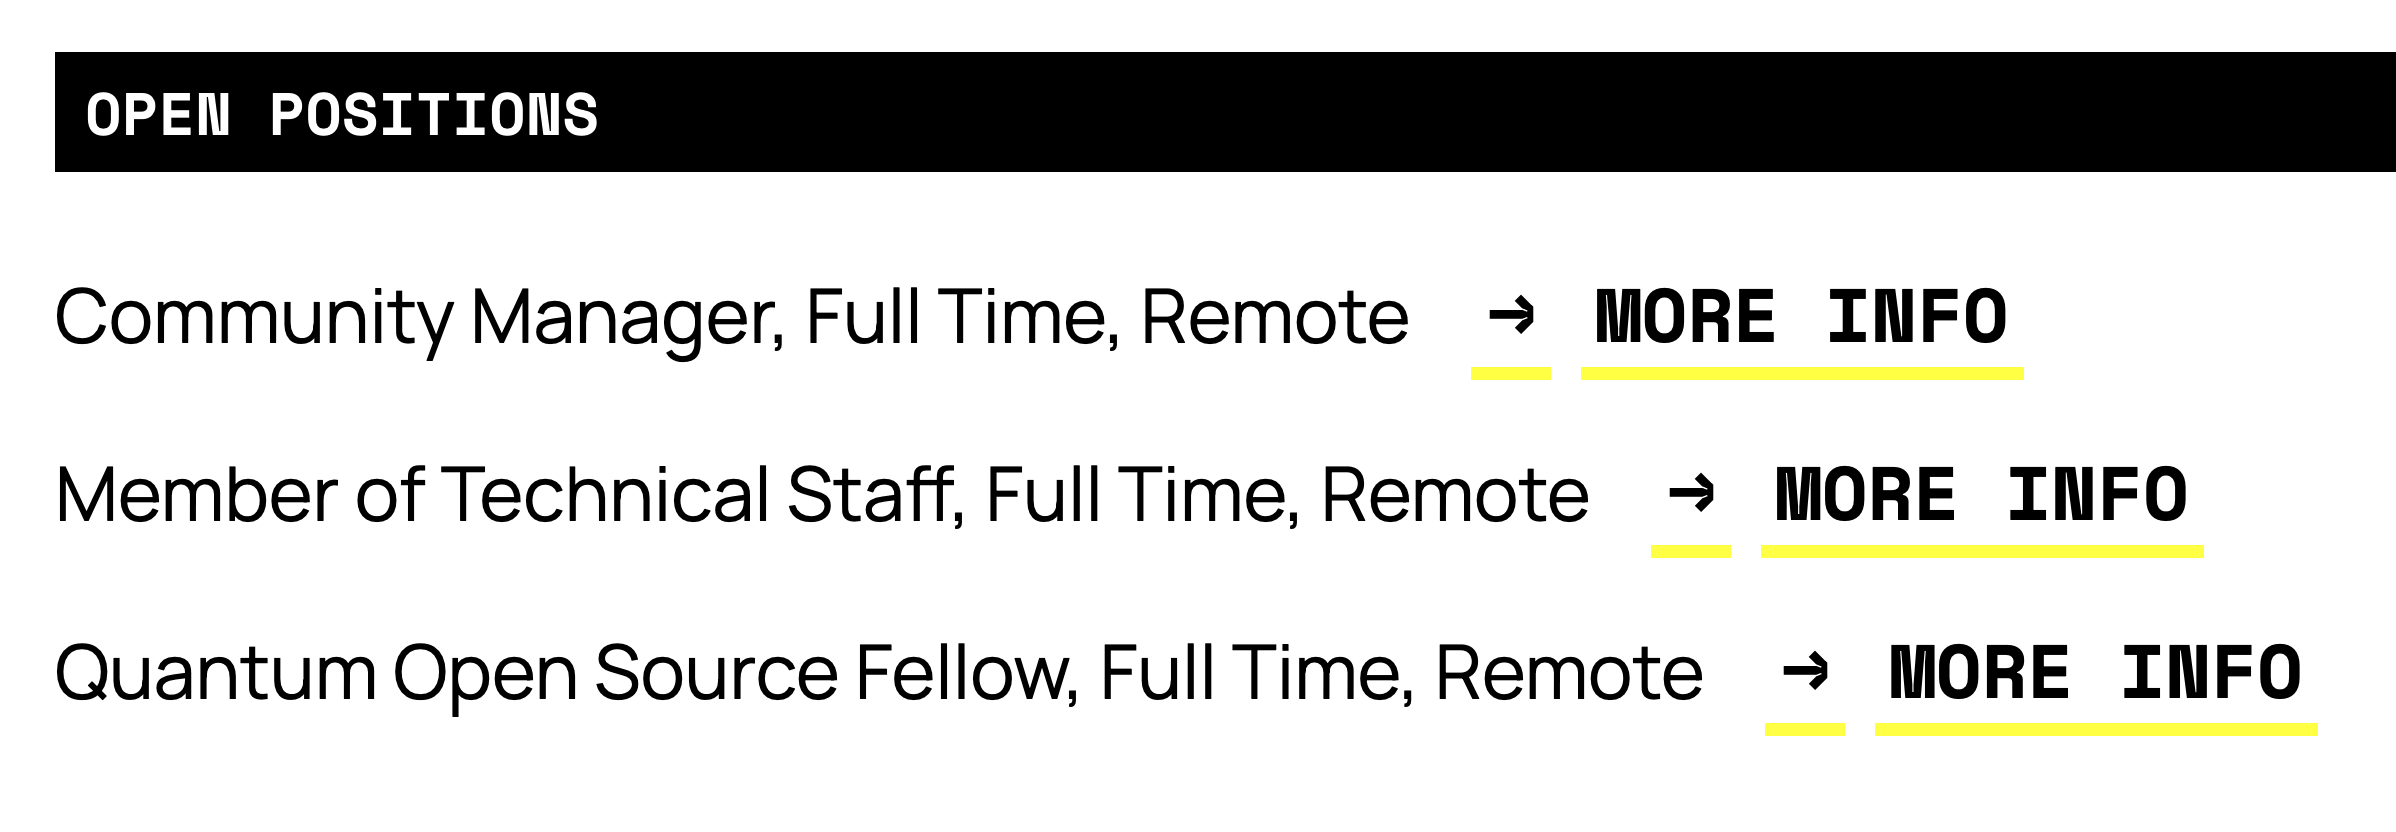
\includegraphics[width=0.7\textwidth]{jobs}
	\end{figure}
	\begin{center}
		\qrcode[height=3cm]{https://unitary.fund/careers/}

		\url{https://unitary.fund/careers/}
	\end{center}
\end{frame}

\end{document}
